% !TEX root=/home/tavant/these/manuscript/src/manuscript.tex

\section{Instability in the \acs{2D} radial-azimuthal \acs{PIC} simulations}
  \label{sec-PIC-ECDI}
  
  \subsection{Introduction and state of the art} \label{subsec-indroECDI}
    
    
    The presence of azimuthal instabilities in the Hall effect thrusters has first been shown with numerical simulations by \citet{adam2004}.
    Then, they have been the subject of numerous studies, especially numerical \citep{ducrocq2006,lafleur2016,lafleur2016a,croes2017,croes2018,janhunen2018,taccogna2019}, but also experimental \citep{honore2011,cavalier2013,cavalier2013a}.
    However, their nature remain unclear \citep{boeuf2018}.

    \vspace{1ex}
    During the three years of my Ph.D., other groups presented new simulation results in similar radial-azimuthal geometries.
    \citet{hara2019a} presents some kinetic simulation results of a \ac{2D} geometry, of size similar to the case studied here.
    However, the authors focused on the electron mobility values, and few information on the instability are given.
    
    In \citet{janhunen2018}, the authors present a collision-less highly resolved \ac{2D} \ac{PIC} simulation.
    No convection and no radial losses compensation models are used, hence the electron energy quickly rises and the density decreases.
    On the other hand, the domain is bigger, with a radial length of $L_r = 53.8\,\milli\meter$ for an azimythal length of $L_{\theta} = 13.45 \,\milli\meter$.
    Three cells by Debye length are used, while there are in average 800 particles per cell.
    In these conditions, the instability rises, but a large radial structure, named Modified Two Stream Instability (MTSI), of wavelength twice as big as $L_r$  is observed.
    
    The simulation parameters of \citet{taccogna2019} are similar to the results presented here, with  $L_r = 15\,\milli\meter$ and $L_{\theta} = 12.5 \,\milli\meter$.
    The results are qualitatively similar to the others, however the authors also observed radial structures, but this time with a wavelength of a third of $L_r$.
        
    \vspace{1ex}
    We can see that the results obtained differ, meaning that some points needs to be clarified.
    Therefore, we present in this chapter the results obtained with \LPPic{}.  
    In \cref{sec-PIC-ECDI}, we present the oscillations observed in the \ac{PIC} simulations.
    After that, we derive the dispersion relation with no hypothesis concerning the particle distribution functions in \cref{sec-DR-kinetic}, and we present in \cref{sec-DR-solver} a numerical algorithm that solves the dispersion relation using the distribution function measured in the \ac{PIC} simulations.
    The oscillations observed in the simulation are compared in \cref{sec-DR-results} to the results of the dispersion relation.
    To finish with; the impact of the radial boundary condition is investigated in \cref{sec-DR-BC}.


  \subsection{Instabilities observed with \LPPic} \label{subsec-lppic_ECDI}
  
  We present in this section the simulation results obtained in one case.
  As we observed the same results when varying the  different physical parameters, for sake of brevity, results for other parameters are not shown.
  The parameters of the simulation are presented in \cref{tab-evdfpicparams}.
  The radial boundary condition includes a dielectric layer of width $L_{diel}$.
  No electron emission is modeled, and the convection is modeled with the new model (see \cref{sec-noiselessresults}).
  
  \begin{table}[!hbt]
  \ra{1.3}
    \centering
    \caption{Parameters of the \acs{2D} \acs{PIC} simulations}
    \label{tab-evdfpicparams}
    \begin{tabular}{@{}r l l l @{}} \toprule
      {\bf Physical Parameter} &  &   &  \\
    Parameter  & notation   &   Value   &  Unit  \\ \midrule
    Dimensions & $L_r\times L_{\theta}\times L_z$   & $1\times 0.26\times 0.5$ & cm \\
    Radial magnetic field & $B_r$  & 0.02 & T \\
    Axial electric field & $E_z$  & \sn{2}{4} & $s\volt\per\meter$ \\
    Dielectric layer of width & $L_{diel}$ & 3 & \milli\meter  \\
    Mean plasma density & $n_{0}$                    & $3 \times 10^{17}$    & {m}$^{-3}$ \\
    Initial electron temperature & $\Te_{,0}  $               & $10.0$                 & V \\
    \midrule
    {\bf Numerical Parameter} &  &   &  \\
    Time step & $\Delta t  $                      & $4 \times 10^{-12}$ & s \\
    Cell size & $\Delta x = \Delta y$ & $2 \times 10^{-5}$  & m \\
    Number of particles per cell & $N/NG      $                      & $80$                & part/cell \\
    \bottomrule
    \end{tabular}
  \end{table}

  \Cref{fig-canon_Te_allch5} shows the temporal evolution of the mean kinetic energy $\Ee$ during the simulations.
  The mean kinetic energy is computed in the simulations by averaging over the whole electron population
  \begin{equation} \label{eq-Ee}
    \Ee_d = \frac{m_e}{2 e N_e} \sum_{j=1}^{N_e} v_{j, d}^2 
  \end{equation}
  with $d$ the direction ($r,\theta$, or $z$), $N_e$ is the number of electron, and $v_{i, d}$ is the velocity in the direction $d$ of the $j^{\rm nt}$ electron.
  We see that the simulation starts at $\Ee = \Te_{,0} /2$, and  that the after a few microseconds of transition, the simulations reaches a steady-state with small fluctuations.
  The correspond to an initial Debye lenght $\lde=\sn{4.3}{-5}\,\meter$ to $\lde=\sn{7.0}{-5}\,\meter$ during the steady state.
  \begin{figure}[!hbt]
    \centering
    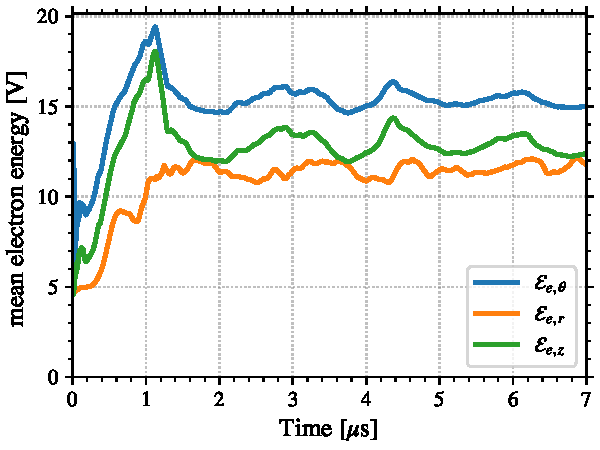
\includegraphics[width=\defaultwidth]{canonical_Te_all_directions.pdf}
    \caption{Temporal evolution of the electron mean kinetic energy decomposed $\Ee$ over the three directions. The kinetic energy include the internal energy (temperature) and the kinetic energy of the mean velocity.}
    \label{fig-canon_Te_allch5}
  \end{figure}
  

  \subsection{General characteristics of the azimuthal instability }
  We focus in this section on the azimuthal instability observed the \ac{2D} \ac{PIC} simulations.
  \Cref{fig-2D_ne} shows the radial-azimuthal distribution of the electron density during the steady state.
  We can see the instability in the azimuthal direction with a wavelength of a third of the azimuthal length.
  The instability can be seen in all of the plasma quantities (electron and ion densities, potential, electric field).
  In the radial direction, we can see the presheaths and the sheaths, characterized by the decrease of the plasma density between the center and the walls.

  \begin{figure}[hbtp]
    \centering
    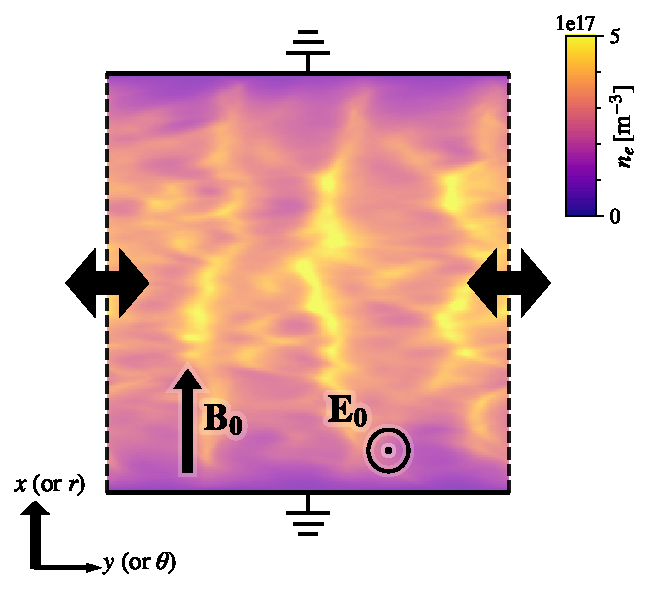
\includegraphics[width=\defaultwidth]{2D_schema_ne}
    \caption{Radial and azimuthal distribution of the electron density $n_e$ at $t=10\,\micro\second$, during the steady state. The azimuthal instability is clearly seen, as well as the sheaths in the radial direction. }
    \label{fig-2D_ne}
  \end{figure}
  
  \Cref{fig-2DcutEx} shows the temporal evolution of the azimuthal electric field and the electron density as a function of the azimuthal position, measured at the center of the radial direction.
  We see the instability growing at the beginning, up to the saturation around $t=1\,\micro\second$.
  Then, we observe, in addition to the fast oscillation, a slower modulation of the oscillation's amplitude, similar to the fluctuations seen in \cref{fig-canon_Te_allch5}.
  \begin{figure}[!hbt]
    \centering
    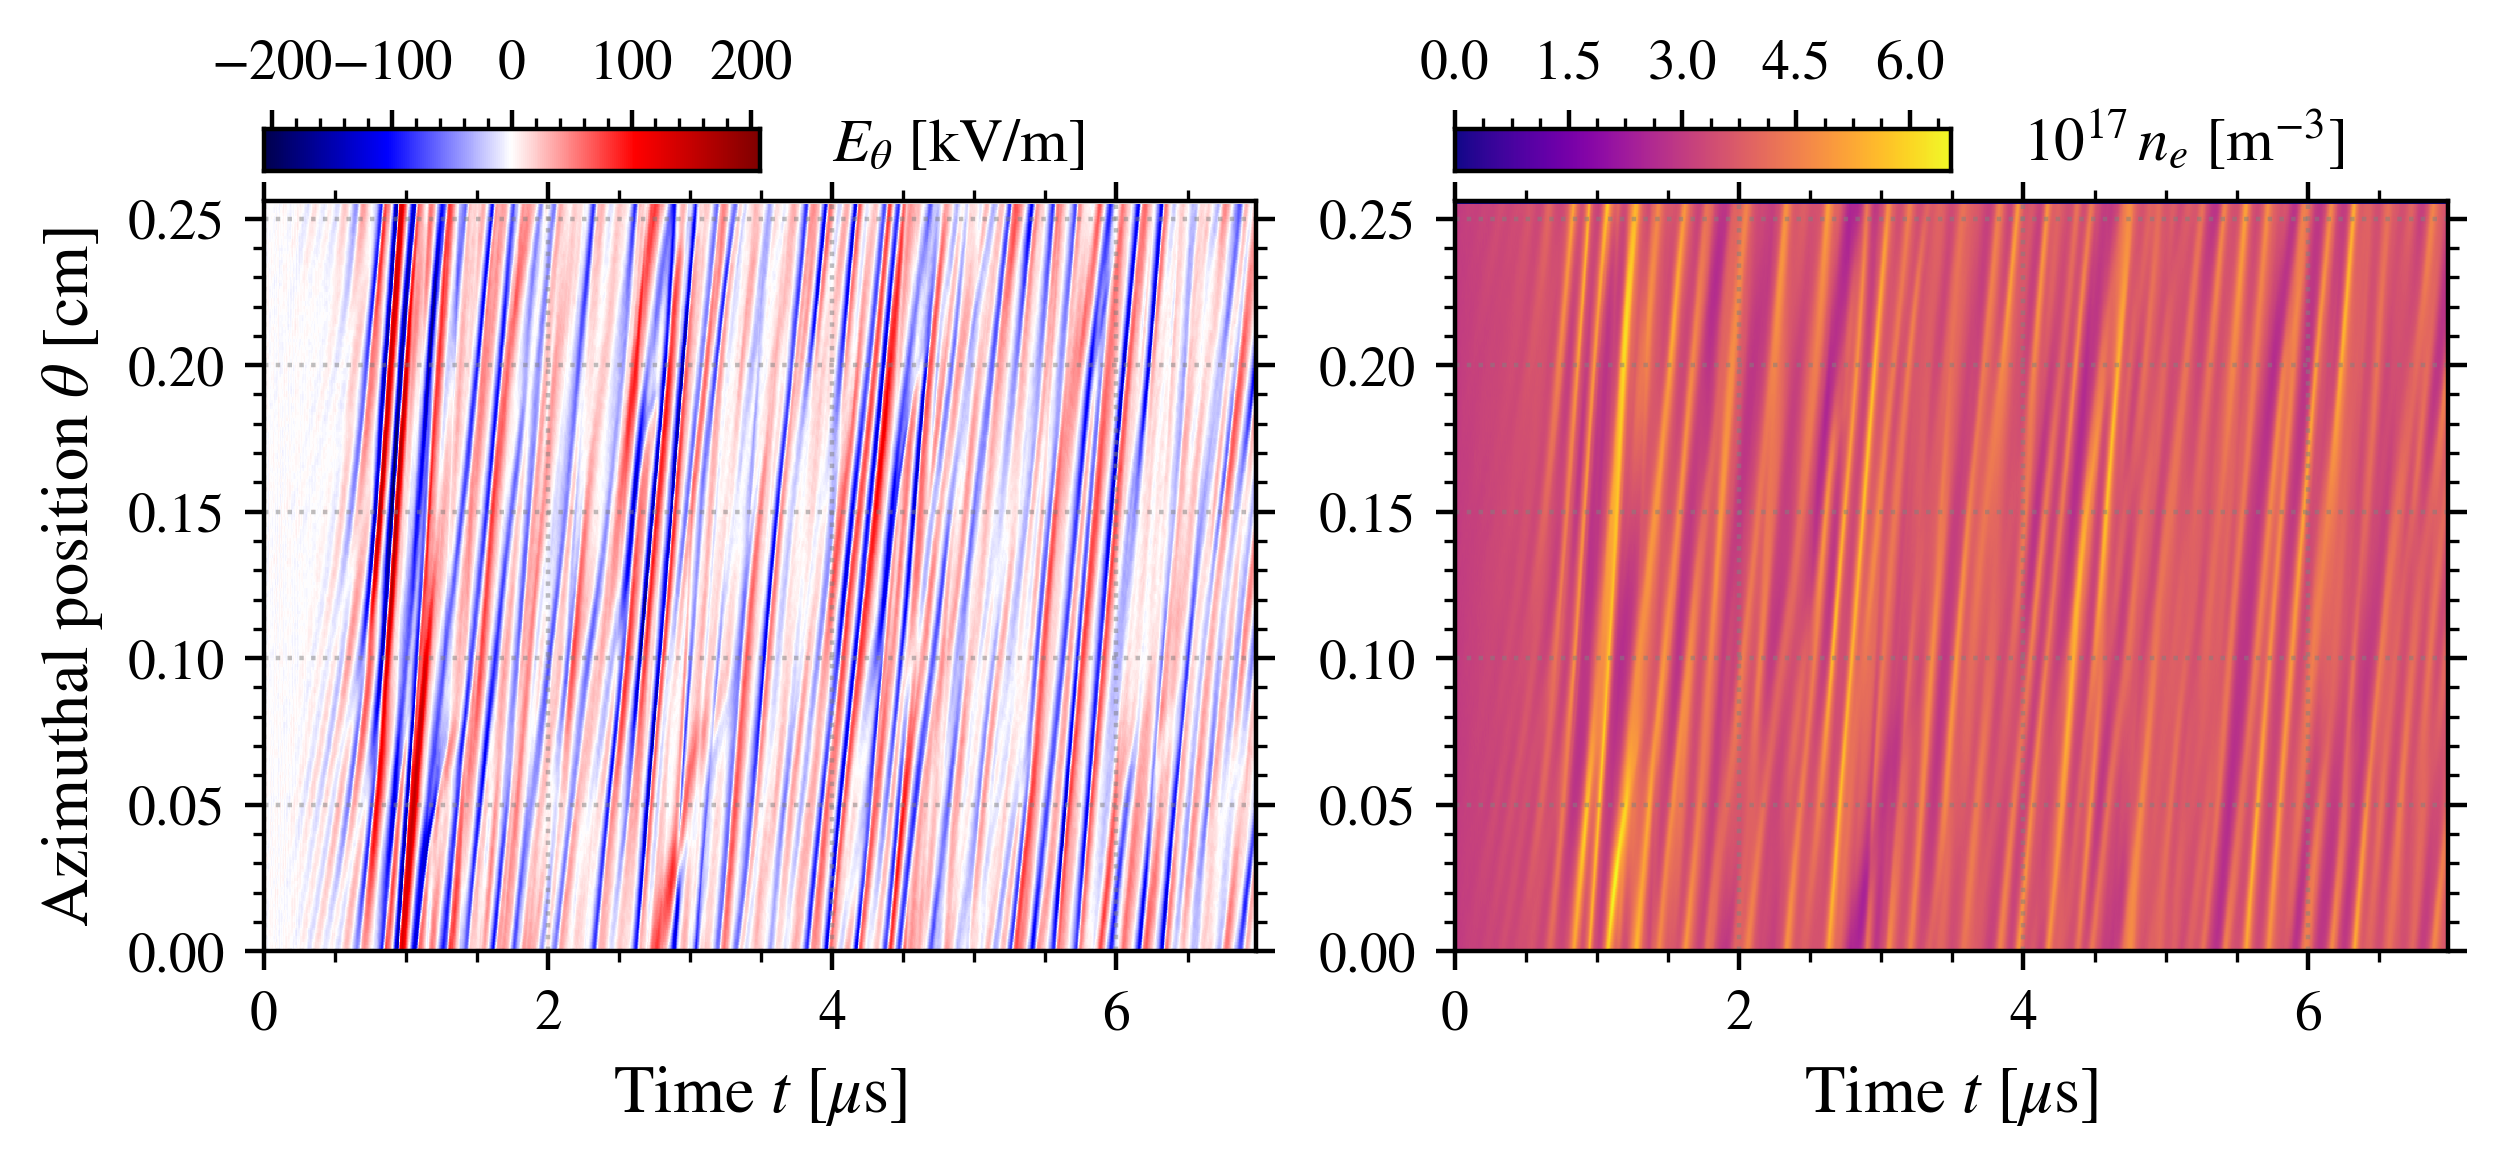
\includegraphics[width=\textwidth]{R_theta_fluctuations}
    \caption{Temporal evolution of (left) the azimuthal electric field $E_{\theta}$, and (right) the electron density $n_e$ as a function of the azimuthal position.}
    \label{fig-2DcutEx}
  \end{figure}

  \Cref{fig-FFT_ex} shows the frequency spectrum of the azimuthal electric field presented in \cref{fig-2DcutEx} computed via \ac{FFT} in the stationary state ($t > 1.2\,\micro\second$).
  The spectrum have been averaged in the azimuthal direction, in order to reduce the noise.
  The theoretical frequency $f_{\rm theo} = \frac{\opi}{\pi \sqrt{6} }$ \citep{croes2018} is given. 
  We can see a very good agreement between $f_{\rm theo}$ and the maximum of the frequency spectrum.
  The value of the theoretical frequency $f_{\rm theo}$ is developed in \cref{sec-DR-kinetic}.
  \begin{figure}[!hbt]
    \centering
    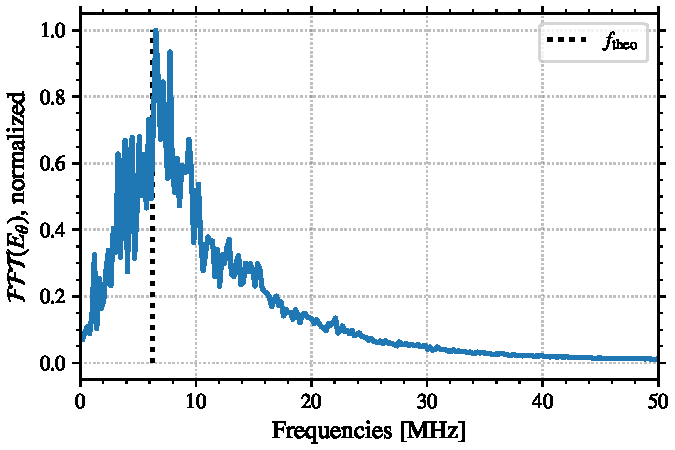
\includegraphics[width=\defaultwidth]{spectrum_frequency}
    \caption{Frequency spectrum of the azimuthal electric field, averaged in the azimuthal direction. The black line is the theoretical frequency.}
    \label{fig-FFT_ex}
  \end{figure}
  
  \subsection{Energy cascade} \label{subsec-turbul}
  
  We can see in \cref{fig-FFT_ex} a slow decrease of the frequency amplitude from $f_{\rm theo}$ to larger frequencies.
  This sort of cascade is typical of turbulences, and can be a source of energy dissipation - hence saturation.
  Kolmogorov's hypothesis of in-compressible fluid leads to a cascade in power law \[ W(f) = | \mathcal{FFT}(E_{\theta})(f) |^2 \propto f ^ {- \alpha}, \]
  with $\alpha = 5/3$.
  
  \begin{figure}[!hbt]
    \centering
    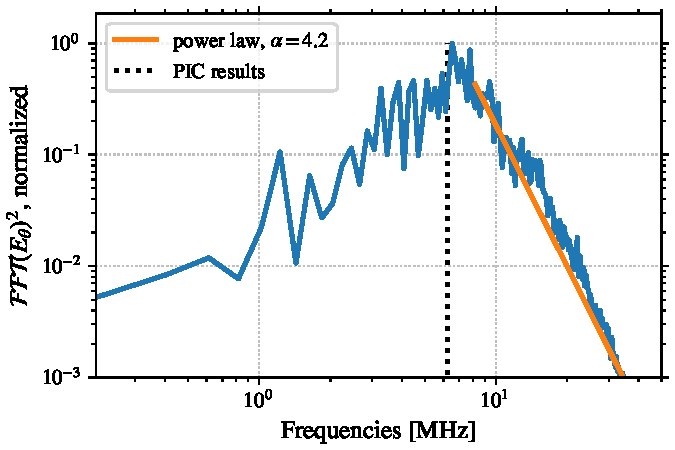
\includegraphics[width=\defaultwidth]{spectrum_frequency_turbul}
    \caption{Normalized frequency power spectrum in log-log scale. The black dotted line shows the  theoretical frequency $f_{\rm theo}$, and the orange solid line is a linear fit of coefficient $\alpha$. }
    \label{fig-turbul}
  \end{figure}
  
  \Cref{fig-turbul} shows the frequency power spectrum in log scale.
  Is overlaid a fit of the cascade, for frequencies above the maximum amplitude.
  The power law obtained is $\alpha \simeq 4.2$.
  The oscillations observed present a decrease of the power spectrum much steeper than expected from turbulence.
  Even if the mechanism of plasma turbulence differs from the fluid turbulence \citep{tsytovich1972}, the value of $\alpha$ is significantly larger than expected, hence we dismiss this phenomenon.
  
  \subsection{Temporal evolution of the oscillation amplitude} \label{subsec-temp}
  We have seen in the previous section that after a growing phase, the amplitude of the instability saturates while oscillates slowly around the stable value.
  This section analyses these temporal characteristics.
  
  \Cref{fig-Ezstd_time} shows the temporal evolution of the characteristics of the electrostatic oscillation.
  As the oscillation is not monochromatic (i.e. it is the sum of multiple waves), we display both the maximum of the electric field $\max(E_{\theta})$, and its standard deviation $\stdE$.
  In the case of a monochromatic wave, one would have 
  \[ \stdE = \frac{\max(E_{\theta})}{\sqrt{2}}.  \]
  
  \begin{figure}[!hbt]
    \centering
    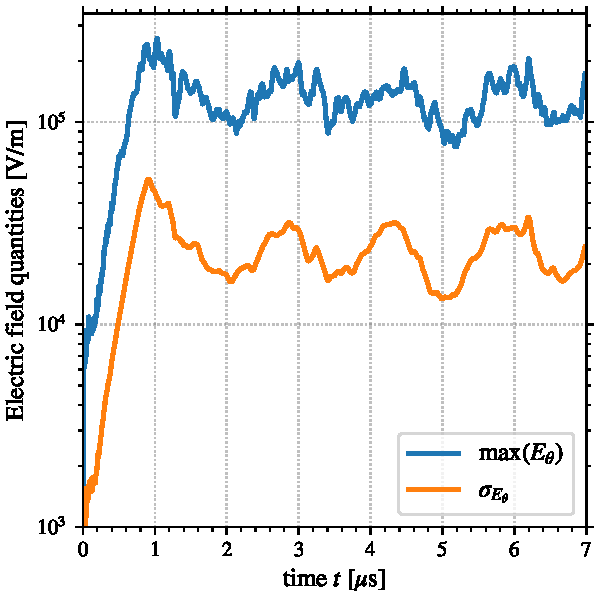
\includegraphics[width=\defaultwidth]{Temporal_E_theta.pdf}
    \caption{Temporal evolution of the maximum and the standard deviation of the azimuthal electric field, in log scale.}
    \label{fig-Ezstd_time}
  \end{figure}
  
  We can see in \cref{fig-Ezstd_time} that during the first microsecond, the growth of the wave amplitude is exponential, corresponding to a constant growth rate.
  A linear fit in log scale give $\gamma_{PIC} \simeq 0.07 \opi$ during the linear phase.
  After $t=1\,\micro\second$, the amplitude of the electric field oscillates around a mean value, with a period of the order of $T_{NL}=1.5 \pm 0.1 \,\micro\second$.
  Hence, the azimuthal electric field becomes of the type of
  \[  E_{\theta} = E_{\rm LF}(t) E_{\rm HF}(t, {\theta}) \]
  with $E_{\rm HF}(t, \theta) $ the high frequency instability, and $E_{\rm LF}(t)$ the modulation of the amplitude, with a low frequency $f_{\rm LF} \simeq  650 \pm 40 \,\kilo\hertz$.
  Several phenomena are candidates to the modulation observed, which are discussed here-after.
  
  
  \paragraph{Ion transit time\\}
    The ions are injected at the anode, and are accelerated by the uniform axial electric field $E_z$.
    The transit time of the ions in the axial direction $T_t$  is the time needed for the ions to travel $L_z$
    \begin{equation} \label{eq-transittime}
      T_{t} = \sqrt{\frac{2 m_i L_z}{e E_z}} \simeq 0.8 \mu s.
    \end{equation}
    
    The transit time is of the good  order of magnitude, but $T_{NL}$ is still twice bigger.
    
  \paragraph{Particle trapping and bouncing\\}
    A common reason for wave saturation is the ion trapping. 
    It has been observed in both \ac{1D} simulation by \citet{lafleur2016a} and in \ac{2D} simulation \citep{croes2017a}.
    Hence, the low frequency modulation could be due to particle bouncing \citep{belmont2013}.
    However, the bouncing time scale is 
    \begin{equation} \label{eq-TB}
      T_{B} = 2 \pi \sqrt{\frac{m_i}{e k \max(E_{\theta})} } \simeq 0.5 \,\micro\second,
    \end{equation}
    which is 3 times smaller than $T_{NL}$.
    Using $\sqrt{2} \sigma_{E_{\theta}}$ instead of $\max(E)$, we find $T_B = 0.9\,\micro\second$
    Even though in \citet{belmont2013}, the authors say that, when the amplitude of the electric field is large (as it is the case here), the bouncing time scale increases due to non-linear phenomenon (the particle trajectory is no longer harmonic), we cannot conclude here that this is the origin of the low frequency modulation.

  
  \paragraph{Ion-wave trapping oscillation\\}
    The wave saturating due to ion-wave trapping has an amplitude of \citep{lafleur2017,boeuf2018}
     \begin{equation} \label{eq-iontropempl}
       \stdE = \frac{\Te}{12 \lde}.
     \end{equation}
    
    Defining the wave energy  density by
    \begin{equation} \label{eq-waveE}
      \epsilon_{\rm wave} = \frac{\epsilon_0}{2} \stdE^2
    \end{equation}
    and the electron thermal energy density with
    \begin{equation} \label{eq-thE}
      \epsilon_{\rm th} = \frac{3}{2} e n_e \Te
    \end{equation}
    
    We find the criterion for the ion-wave trapping
    \begin{equation} \label{eq-criteriaIT}
      432 \epsilon_{\rm wave} = \epsilon_{\rm th}.
    \end{equation}
    
    \Cref{fig-tempITcrit} shows the temporal evolution of the electron thermal energy $\epsilon_{\rm th}$ and the wave energy density $\epsilon_{\rm wave}$, scaled by the factor 432.
    We can see that $\epsilon_{\rm th}$ is relatively constant.
    However, $\epsilon_{\rm wave}$  oscillates significantly, and passes regularly above and below $\epsilon_{\rm th}$.
    
    \begin{figure}[!hbt]
      \centering
      % 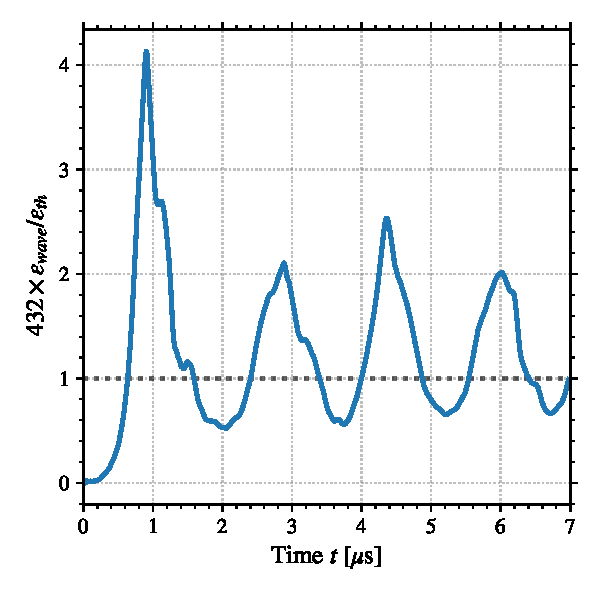
\includegraphics[width=\defaultwidth]{Ion_Trapping_criter}
      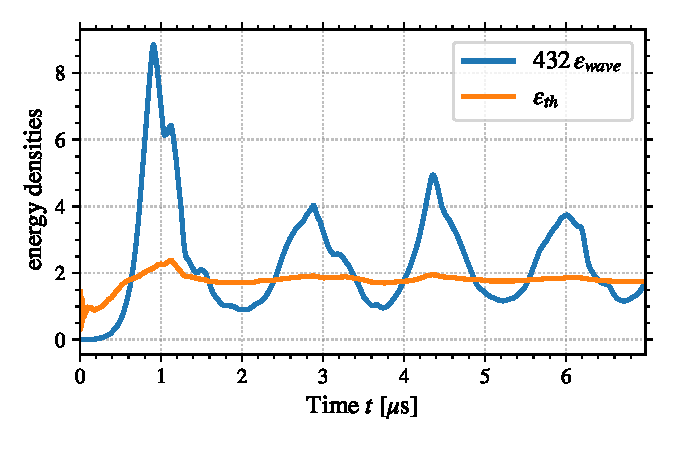
\includegraphics[width=\defaultwidth]{Ion_Trapping_criter_bis}
      \caption{Temporal evolution of the wave energy density (scaled) compared to the thermal energy density.}
      \label{fig-tempITcrit}
    \end{figure}
    
    In \cref{fig-tempITcrit}, as expected the period of the oscillations of $\epsilon_{\rm wave}$ is $T_{NL} = 1.5\,\micro\second$.
    But here, we can see that when the criterion \cref{eq-criteriaIT} is fulfilled, the temporal derivative of the growth rate is positive.
    However, a delay $\tau$ after the moment when the criterion is violated ($\tau = 0.40 \pm 0.07 \,\micro\second$ on the four oscillations), the wave abruptly stops rising and decreases instead.
    This delay between the time the ions should be trapped and the time the wave stops growing in most certainly due to the ion inertia, as we have $\tau \sim T_B$.
    
    To summarized, the low frequency modulation of the azimuthal wave amplitude is certainly due to non-linear behavior of wave-particle interaction.
    Complementary results are presented in \cref{subsec-VDFIAW} by solving the dispersion relations.
    
